% !TEX root = ThesisGchatzi.tex

\graphicspath{{Papers/SSTD2019/}{Papers/SIGSpatial2019/}}

In this chapter, we introduce the measure of \textit{local similarity}, that can be applied on co-evolving (i.e., time aligned) time series. Two co-evolving time series are locally similar if the pairwise distance of their values per timestamp does not exceed a given threshold during a time interval, that lasts at least a pre-defined number of consecutive timestamps. Based on this new similarity measure, we introduce two novel approaches for efficiently detecting all possible pairs and \textit{bundles} (groups) of time series that are locally similar within a given dataset. Additionally, we utilize our hybrid \btsr index to answer several hybrid queries on geolocated time series based on local similarity and introduce an extension to \btsr, named \sbtsr that significantly speeds up the process.

The bundle discovery problem we address in this Thesis resembles the problem of \textit{flock discovery in moving objects}, where the goal is to identify sufficiently large groups of objects that move close to each other over a sufficiently long period of time. However, to the best of our knowledge, ours is the first work to address the problems of locally similar pair and bundle discovery over co-evolving time series. 

\paragraph{Local Pair and Bundle Discovery.} Discovering such pairs and bundles is useful in various applications. For instance, public utility companies employ smart meters to collect time series measuring consumption per household (e.g., for water or electricity). Identifying such bundles of time series (i.e., a number of similar subsequences over certain time intervals) can reveal similar patterns of consumption among users, allowing for more personalized billing schemes. In finance, examining time series of stock prices can identify pairs or bundles of stocks trending similarly at competitive prices over some trading period, hence offering precious insight for possible future investments.

\begin{figure}[b]
    \centering
    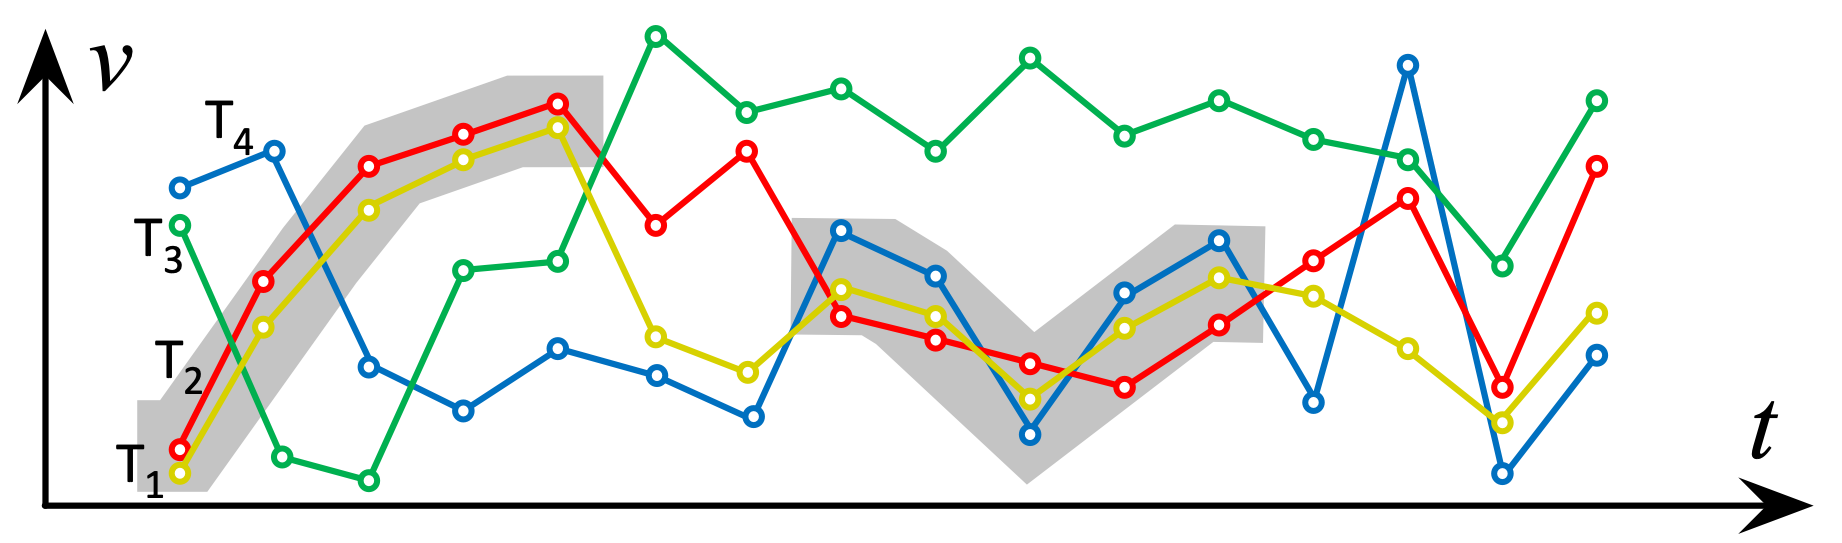
\includegraphics[width=0.75\textwidth]{figures/pair_flock_ex.png}
    \caption{A pair and a bundle of locally similar time series.}
    \label{fig:pair_flock_ex}
\end{figure}

Figure~\ref{fig:pair_flock_ex} illustrates an example comprising four time series depicted with different colors. We observe that from timestamp 1 to 5 the values of $T_1$ and $T_2$ are very close to each other, thus forming a locally similar pair. Similarly, from timestamp 8 to 12, the values of $T_1$, $T_2$ and $T_4$ are close to each other, forming a bundle with three members. Note that values in each qualifying subsequence may fluctuate along a bundle as long as they remain close to the respective values per timestamp of the other members in that bundle.

A real-world example is depicted in Figure~\ref{fig:water_real_ex}. These two time series represent per-hour average water consumption during a day of the week for two different households. We can observe that their respective values per timestamp (at granularity of hours, in this example) are very close to each other during a certain time period (hours 2-11), but are farther apart in the rest. Hence, an algorithm that measures the global similarity between two time series might not consider this pair as similar; however, the subsequences inside the gray strip are clearly pairwise similar, and might indicate an interesting pattern. Identifying such local similarities within a sufficiently long time interval is our focus in this chapter.

\begin{figure}[tb]
    \centering
    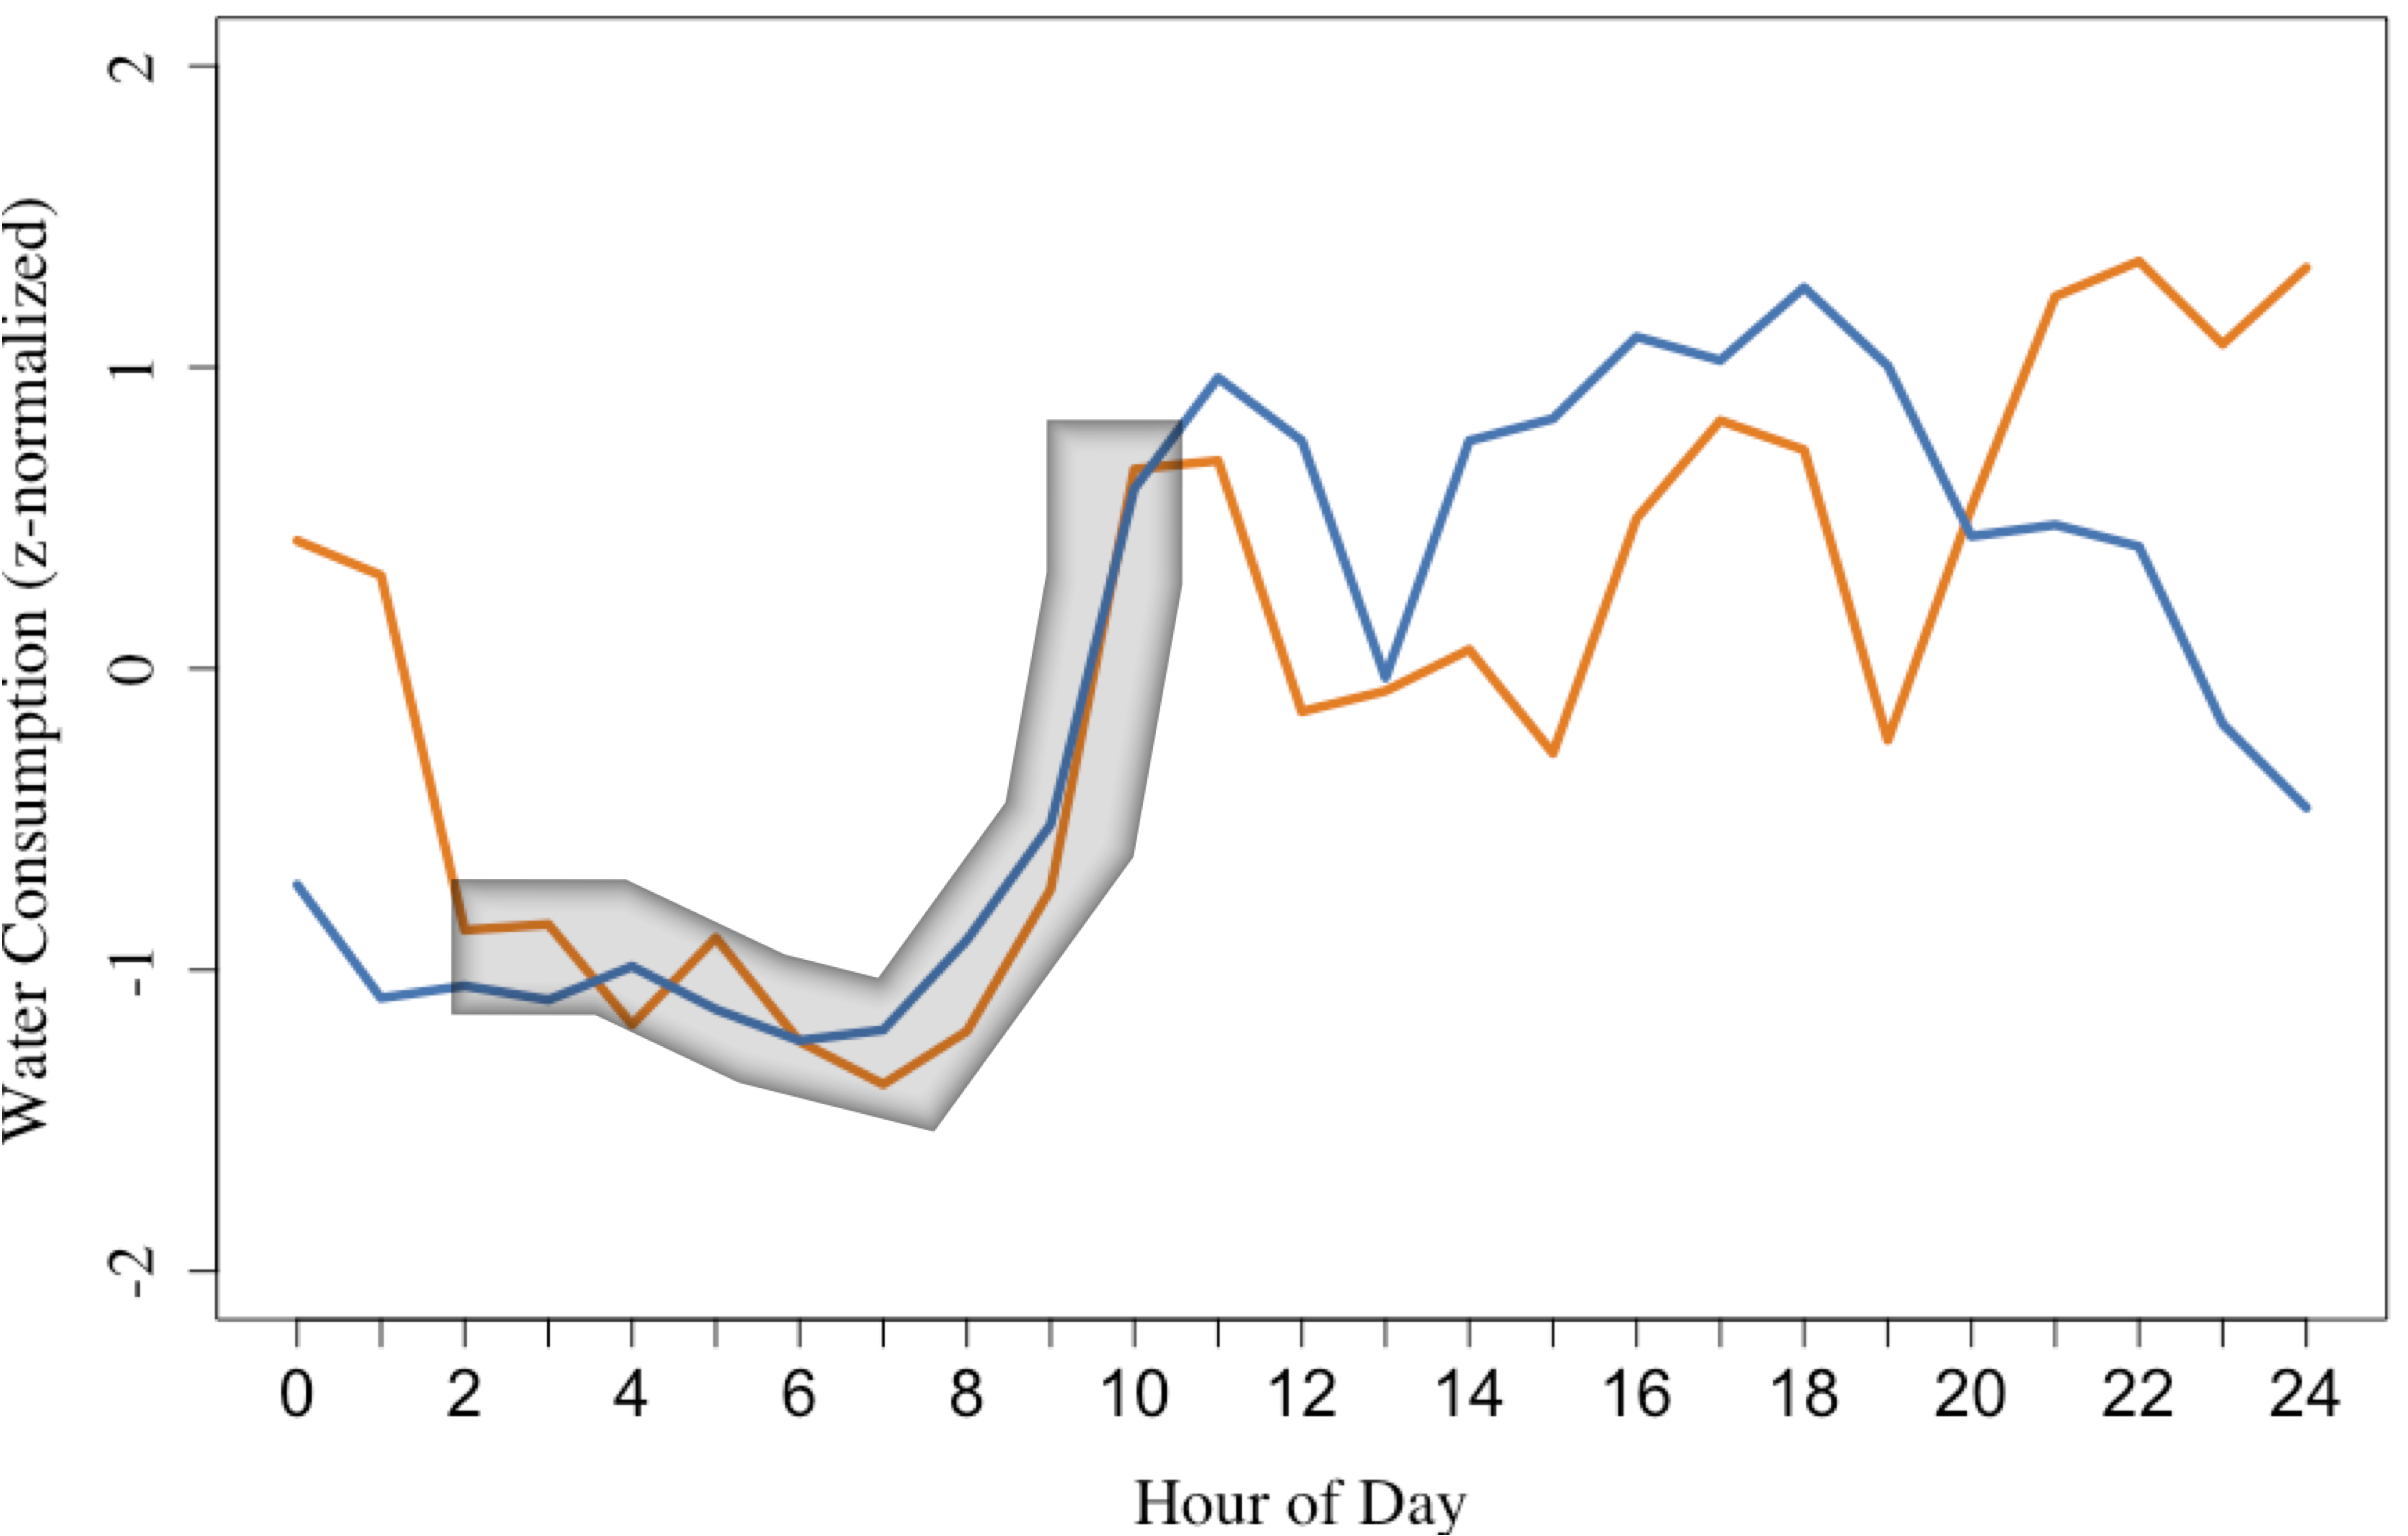
\includegraphics[width=0.75\textwidth]{figures/water_real_ex.png}
    \caption{Pair of locally (but not globally) similar time series.} 
    \label{fig:water_real_ex}
\end{figure}

Furthermore, Figure \ref{fig:bundles_water} depicts several bundles of locally similar time series detected by our algorithms in a real-world dataset containing smart water meter measurements. The detected bundles represent different per-hour average water consumption patterns during a week. There is a wider pattern detected among 6 households during the first 30 hours of the week indicating reduced consumption (probably no permanent residence). The orange and yellow patterns indicate different morning routines during the third and fourth day of the week. The green and purple patterns represent a reduction in consumption during the late hours of the fourth and sixth day, respectively, with some intermediate consumption taking place during the night. Finally, the shorter red and light blue bundles suggest different evening patterns for two other days (respectively, decreasing and increasing consumption).

\begin{figure}[tb]
    \centering
    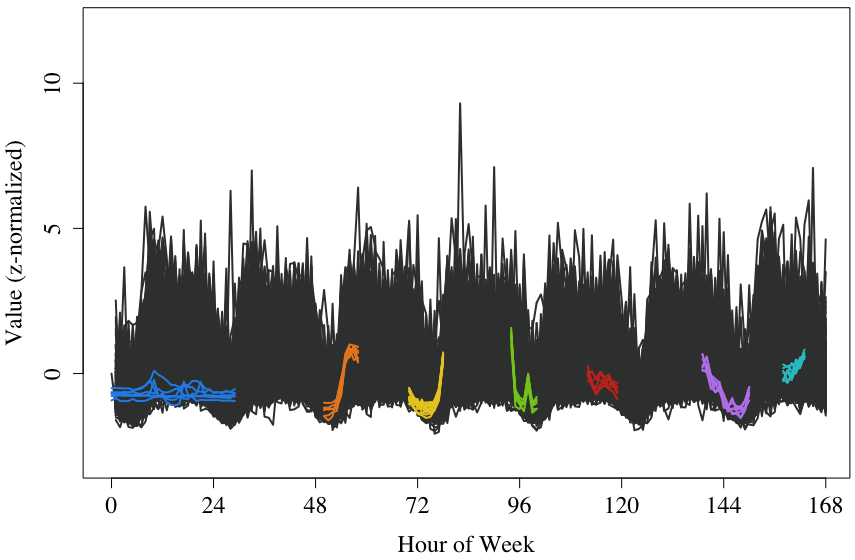
\includegraphics[width=0.75\textwidth]{figures/bundles_water.png}
    \caption{Bundles of locally similar time series.}
    \label{fig:bundles_water}
\end{figure}

%Challenges
Discovering all possible pairs and bundles of locally similar time series, along with the corresponding subsequences, within large sets is a computationally expensive process. To find matches, a filter-verification technique can be applied. At each timestamp, the {\em filtering} step can discover candidate pairs or groups having values close to each other; then, the {\em verification} step is invoked to determine whether each such candidate satisfies the required conditions, essentially whether this match occurs throughout a sufficiently large time interval. However, both the filtering and the verification steps are expensive. The computational cost becomes especially high for the case of bundle discovery, as it has to examine all possible subsets of locally similar time series that could form a bundle. Hence, such an exhaustive search is prohibitive when the number and/or the length of the time series is large.

%General approach
We employ a value discretization approach that divides the value axis in ranges equal to the value difference threshold $\epsilon$, in order to reduce the number of candidate pairs or bundles that need to be checked per timestamp. Leveraging this, we first propose two \textit{sweep line} scan algorithms, for pair and bundle discovery respectively, which operate according to the aforementioned filter-verification strategy. However, this process still incurs an excessive amount of comparisons, as it needs to scan all values at every timestamp. To overcome this, we introduce a more aggressive filtering  that only checks at selected \textit{checkpoints} across time, but ensuring that no false negatives ever occur. This approach incurs significant savings in computation cost, as we only need to examine candidate matches on those checkpoints only instead of all timestamps. To further reduce the number of examined candidates, we propose a strategy that judiciously places these checkpoints across the time axis in a more efficient manner. We then exploit these optimizations introducing two more efficient algorithms that significantly reduce the execution cost for both pair and bundle discovery.

The bundle discovery problem we address in this chapter resembles the problem of \textit{flock discovery in moving objects}, where the goal is to identify sufficiently large groups of objects that move close to each other over a sufficiently long period of time \cite{gudmundsson2006computing, benkert2008reporting, vieira2009line, tanaka2015efficient}. In fact, the baseline algorithm we describe can be viewed as an adaptation of the algorithm presented  in \cite{vieira2009line}. However, to the best of our knowledge, ours is the first work to address the problems of locally similar pair and bundle discovery over co-evolving time series. 

\paragraph{Local Similarity Search on Geolocated Time Series.} Our approach for hybrid search over geolocated time series (see \ref{chap:btsr}) using the \btsr supports only {\em global} time series similarity, i.e., similarity measured across the entire length of time series. Specifically, as in other works in this area \cite{DBLP:journals/pvldb/EchihabiZPB18,jessica2007dmkd,camerra2010icdm,camerra2014kais}, the distance between two time series is measured by aggregating the pairwise Euclidean distance of their respective values across the entire sequences. However, in many cases, more fine-grained trends and patterns may exist, which are missed under this global similarity measure. For example, consider two time series representing the hourly energy consumption of two nearby buildings over a week, and assume that the two buildings exhibit a similar consumption pattern during working days but a different one in weekends. A query imposing a similarity threshold over the entire week would fail to identify these two geolocated time series as similar. However, it may be useful to discover that there is a period of up to 5 days during which these two time series are actually similar.

Motivated by this observation, in this work we extend our previous approach on hybrid queries over geolocated time series to support {\em local similarity} of time series, thus allowing more flexible and fine-grained queries and analyses. The {\em local similarity score} between two time series $T_i$ and $T_j$ is defined as the maximum number of consecutive timestamps during which the respective values of $T_i$ and $T_j$ do not differ by more than a user-specified threshold $\epsilon$. Notice that, compared to global similarity, this condition is more relaxed, in the sense that it is applied to subsequences of length lower than $T_i$ and $T_j$, but at the same time stricter, in the sense that the threshold $\epsilon$ is required to be satisfied at each individual timestamp during the selected period rather than on the aggregate distance over all timestamps.

Combining this local similarity constraint with a filter on {\em spatial distance} leads to a novel set of hybrid queries. Figure~\ref{fig:example_query} shows an example with a query time series $T_q$ searching over a set of time series $T_1,\dots,T_9$ for those within radius $\rho$ from its location and also locally similar to $T_q$. In particular, with respect to a given $\epsilon$, results should also be locally similar to $T_q$ for at least 5 consecutive timestamps. Qualifying results include $T_2$ with local similarity score $\sigma_2 = 5$ (bottom chart), and $T_7$ with $\sigma_7 = 7$ (top chart).

\begin{figure}[!t]
 \centering
 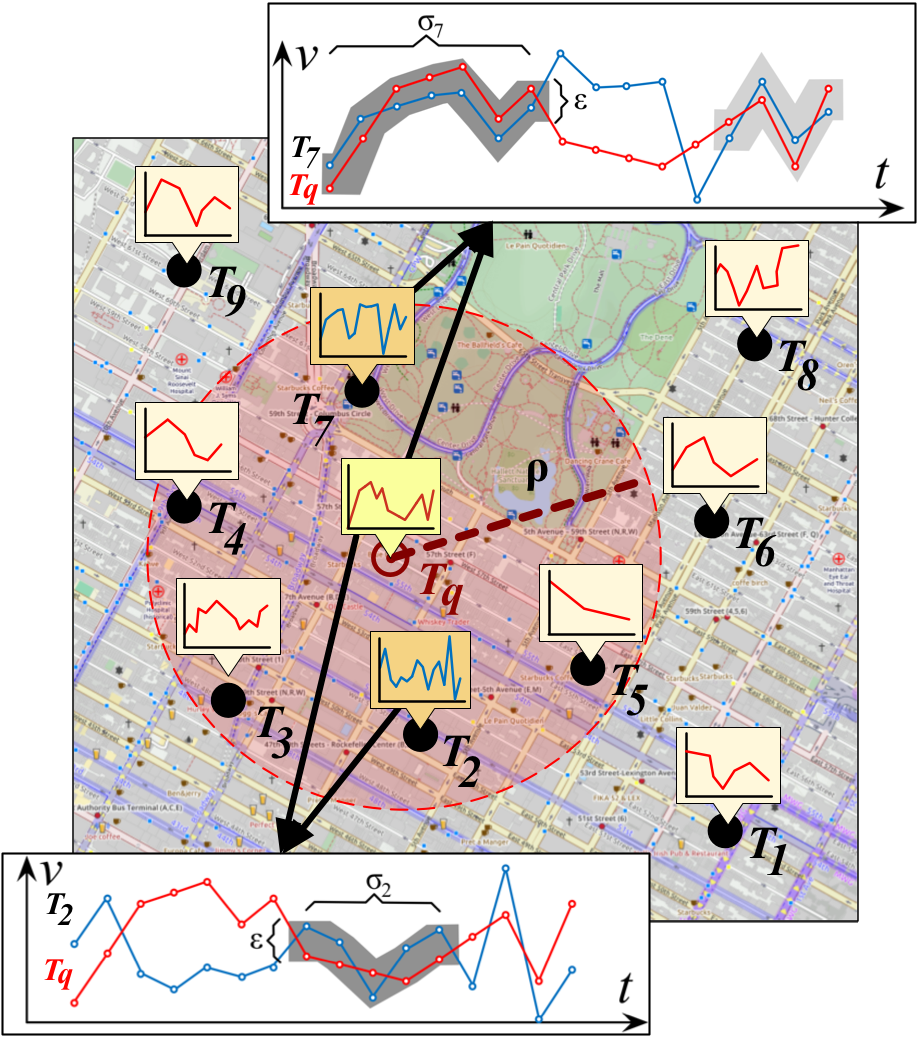
\includegraphics[width=0.5\textwidth]{Figures/local_sim_geoloc.png}
\caption{Retrieving geolocated time series based on spatial distance and local similarity.}
\label{fig:example_query}
\end{figure}

It turns out that such hybrid queries involving local similarity can still be evaluated using the \btsr index. We first present a baseline method employing a sweep-line algorithm to check for local similarity, and then describe how this can be optimized by using appropriately placed {\em checkpoints}, based on the local similarity score threshold specified by the query, in order to skip unnecessary comparisons. Despite the fact that this saves some computations, the resulting time savings are relatively small, since the number of index nodes that need to be probed is not essentially reduced. To overcome this problem, we introduce an improvement to the \btsr index, which is based on temporally segmenting the time series bounds within each node and deriving tighter bounds per segment. Once the time series bounds in each node become more fine-grained, pruning the search space for local similarity queries proves much more effective.

The rest of this chapter is organized as follows. For pair and bundle discovery, Section \ref{subsec:local_sim_join_problem} describes the problems. Sections \ref{subsec:local_sim_join_methods} and \ref{subsec:local_sim_join_bundle} introduce our algorithms and Section \ref{subsec:local_sim_join_exp} reports our experimental results. For local similarity search on geolocated time series, Section~\ref{subsec:local_sim_search_problem} formally defines the problem. Section~\ref{subsec:local_sim_search_methods} presents how query evaluation under local time series similarity can be executed using the \btsr. Then, Section~\ref{subsec:sbtsr_index} presents the enhanced \sbtsr. Section~\ref{subsec:local_sim_search_exp} reports our experimental results. Finally, Section~\ref{sec:concl_local_sim} concludes this chapter.